%%%%%%%%%%%%%%%%%%%%%%%%%%%%%%%%%%%%%%%%%%%%%%%%%%%%%%%%%%%%%%%%%%%%%%%%
%%%%%%%%%%%%%%%%%%%%%%% THEORETICAL REVIEW %%%%%%%%%%%%%%%%%%%%%%%%%%%%%
%%%%%%%%%%%%%%%%%%%%%%%%%%%%%%%%%%%%%%%%%%%%%%%%%%%%%%%%%%%%%%%%%%%%%%%%

In this chapter, we introduce the theoretical concepts used along this thesis. The definitions below are derived from the works of Rozenberg et al., Janssens, and Kim \cite{rozenberg1986boundary, janssens1982graph,kim2001efficient}.
We first go on to define graphs and graph grammars and then, building upon it, we construct the so-called triple graph grammars and discuss the parsing of graphs with graph grammars.

%%%==================================================================%%%
%%%%%%%%%%%%%%%%%%%%%%%%%%% GRAPH GRAMMARS %%%%%%%%%%%%%%%%%%%%%%%%%%%%%
%%%==================================================================%%%
\section{Graph Grammars}
We start presenting our notation for graphs and graph grammars, accompanied by examples, then we introduce the dynamic aspects of the graph grammar formalism, what allows us to comprehend how it can be used for transformation of models.

%%%%%% Abstract Syntax %%%%%%
\begin{definition}
	\label{def:graph}
	A \emph{directed labeled graph} $G$ over the finite set of symbols $\Sigma$, $G = (V, E, \phi)$ consists of a finite set of vertices $V$, a set of labeled directed edges $E \subseteq V \times \Sigma \times V$ and a vertex labeling total function $\phi : V \to \Sigma$.
\end{definition}

Directed labeled graphs are often referred to simply as graphs. For a fixed graph $G$ we refer to its components as $V_G$, $E_G$ and $\phi_G$. Moreover, we denote the set of all graphs over $\Sigma$ by $\allgraphs{\Sigma}$. In special, we do not allow loops (vertices of the form $(v,l,v)$), but multi-edges with different labels are allowed.

If $\phi_G(v) = a$ we say $v$ is labeled by $a$. Two vertices $v$ and $w$ are neighbors (also adjacent) if, and only if, there is one or more edges between them, that is, $(v,l,w) \in E_G$ or $(w,l,v) \in E_G$, for any symbol $l$. Two graphs $G$ and $H$ are disjoint if, and only if, $V_G \cap V_H = \emptyset$. For two graphs $G$ and $H$, we write $G \subseteq H$ if, and only if, $V_G \subseteq V_H, E_G \subseteq E_H$ and $\phi_G \subseteq \phi_H$

We define also the function $\neigh{G}: 2^{V_G} \to 2^{V_G}$, that applied to $U$ gives the set of neighbors of vertices in $U$ minus $U$. That is $\neigh{G}(U) = \{ v \in V_G \setminus U \st \text{ exists a } (v,l,u) \in E_G \text{ or a } (u,l,v) \in E_G \text{ with } u \in U \}$

\begin{definition}
	\label{def:morphism}
	A \emph{morphism} of graphs $G$ and $H$ is a mapping $m: V_G \to V_H$.
\end{definition}

\begin{definition}
	An \emph{isomorphism} of directed labeled graphs $G$ and $H$ is a bijective mapping $m: V_G \to V_H$ that maintains the connections between vertices and their labels, that is, $(v,l,w) \in E_G$ if, and only if, $(m(v),l,m(w)) \in E_H$ and $\phi_G(v) = \phi_H(m(v))$. In this case, $G$ and $H$ are said to be isomorphic, we write $G \isomorph H$, and we denote the equivalence class of all graphs isomorphic to $G$ by $[G]$.
\end{definition}

Notice that, contrary to isomorphisms, morphisms do not require bijectivity nor label or edge-preserving properties.

We use graphs to represent models, first, because of the extensive theory behind graphs and, second, because graphs suit the description of a large spectrum of practical models well, due to their very abstract nature. In the following, we introduce graph grammars, which also suit our needs very well. This is because they can characterize (possibly infinite) sets of graphs using very few notation.

\begin{definition}
	\label{def:gg}
	A \emph{graph grammar with neighborhood-controlled embedding} (NCE graph grammar) $GG = (\Sigma, \Delta \subseteq \Sigma, S \in \Sigma, P)$ consists of a finite set of symbols $\Sigma$ that is the alphabet, a subset of the alphabet $\Delta \subseteq \Sigma$ that holds the terminal symbols (we define the complementary set of non-terminal symbols as $\Gamma := \Sigma \setminus \Delta$), a special symbol of the alphabet $S \in \Sigma$ that is the start symbol, and a finite set of production rules $P$ of the form $(A \pro R, \omega)$ where $A \in \Gamma$ is the so-called left-hand side, $R \in \allgraphs{\Sigma}$ is the right-hand side and $\omega : V_R \pto 2^{\Sigma \times \Sigma}$ is the partial embedding function from the $R$'s vertices to pairs of edge and vertex labels.
\end{definition}

A production rule $(A \pro R, \omega)$ can be applied on a graph $G$ to generate another graph $H$. In this case, we say $G$ \textit{concretely derives in one step into} $H$. This concrete derivation can be informally understood as the replacement of a $A$-labeled vertex $v$ and all its adjacent edges in $G$ by the graph $R$ plus edges $e$ between former neighbors $w$ of $v$ and some vertices $t$ of $R$, provided $e$'s label and $w$'s label are in the embedding specification $\omega(t)$. That is, the embedding function $\omega$ of a rule specifies which neighbors of $v$ are to be connected with which vertices of $R$, according to their labels and the adjacent edges' labels. The process that governs the creation of these edges is called embedding and can occur in various forms in different graph grammar formalisms. We opted for a rather simple approach, in which the edges' directions and labels are maintained. As an additional note, it is worth mentioning, that string grammars have no embedding because a replaced symbol in a string has ``connections" only with its left and right neighbors, so the replacement is always ``connected" with both sides.

Figure \ref{fig:rule-application} illustrates the concrete derivation of $G$ into $H$ with rule $r = (A \pro R, \omega)$ and vertex $v$, with $\omega = \{u \mapsto \{(m,b),(k,c)\} \st w \in V_R\}$. In the upper part of the figure, $G$ containing the $A$-labeled vertex $v$ undergoes the rule application and generates $H$ with the subgraph $R$. In the left bottom part, the context of $v$ with its two adjacent vertices labeled by $b$ and $c$ with edges $m$ and $k$, respectively, is highlighted. On the right bottom, the same context connected to the graph $R$ is displayed. Both contexts are equal because the embedding function $\omega$ enables that all $b$-labeled adjacent vertices of $v$ with a $m$-labeled edge and all $c$-labeled adjacent vertices of $v$ with $k$-labeled edge to be connected to all vertices of $R$. At this point, it is clear that both contexts could differ depending on the embedding function $\omega$. Also notice that it is not guaranteed that the amount of edges be equal in both contexts, for an edge in $G$ can produce more than one edge in $H$.

\begin{figure}
	\centering
	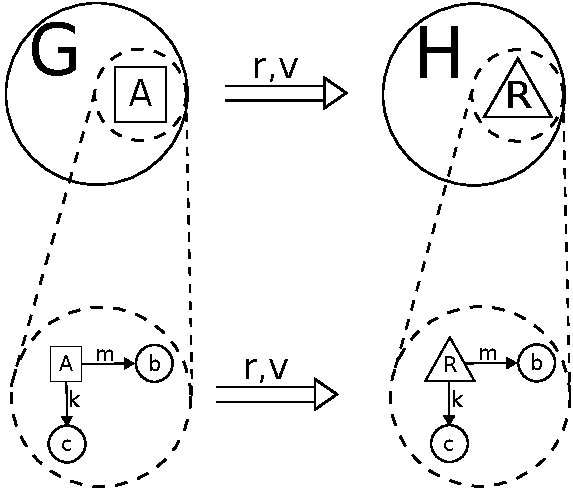
\includegraphics[width=.5\textwidth]{figures/misc/rule-application}
	\caption{Application of the rule $r = (A \pro R, \omega)$ on the graph $G$ and $A$-labeled vertex $v$ that generates graph $H$ containing the subgraph $R$ that is embedded in it according to the embedding function $\omega$. In detail below, the context in $G$ of the vertex $v$ with its two adjacent vertices labeled by $b$ and $c$, as well as, the context of the subgraph $R$ in $H$ with the same adjacent vertices are highlighted.}
	\label{fig:rule-application}
\end{figure}

NCE graph grammars are often referred to as graph grammars or simply as grammars. Vertices from the right-hand sides of rules labeled by non-terminal (terminal) symbols are said to be non-terminal (terminal) vertices and although we do not distinguish between edges labeled with a terminal or a non-terminal symbol, all edges are, in practice, expected to be labeled with a terminal symbol, since edges always maintain their labels throughout rule applications.

Notice that, in the original definition of NCE grammars \cite{janssens1982graph}, the left-hand side of the productions were allowed to contain any connected graph. So, strictly speaking, the definition above characterizes actually a 1-edNCE graph grammar, that contains only one element in the left-hand side and a directed edge-labeled graph in the right-hand side. Nevertheless, for simplicity, we use the denomination NCE to mean a 1-edNCE grammar.

%%%%%% Semantics %%%%%%
In the sequel, we introduce, formally, how production rules are applied to graphs and expose, by means of the concepts of concrete derivation step, derivation step, derivation and language, the dynamic aspects of NCE graph grammars.

\begin{definition}
	\label{def:gg_dstep}
	Let $GG = (\Sigma, \Delta, S, P)$ be a graph grammar and $G$ and $H$ be two graphs over $\Sigma$ that are disjoint to all right-hand sides from $P$, $G$ \emph{concretely derives in one step into} $H$ with rule $r$ and vertex $v$, we write $G \cderiv{r}{v}{GG} H$ and call it a \emph{concrete derivation step}, if, and only if, the following holds:
	\begin{align*}
		r & = (A \pro R, \omega) \in P \text{ and } A = \phi_G(v) \text{ and} \\
		V_H  & = (V_G \setminus \{v\}) \cup V_R \text{ and} \\
		E_H & = (E_G \setminus (\{(v,l,w) \st (v,l,w) \in E_G\} \cup \{(w,l,v) \st (w,l,v) \in E_G\})) \\
		& \cup E_R \\
		& \cup \{(w,l,t) \st (w,l,v) \in E_G \land (l,\phi_G(w)) \in \omega(t)\} \\
		& \cup \{(t,l,w) \st (v,l,w) \in E_G \land (l,\phi_G(w)) \in \omega(t)\} \text{ and} \\
		\phi_H & = (\phi_G \setminus \{(v,x) \st x \in \Sigma \}) \cup \phi_R
	\end{align*}
\end{definition}

Notice that, without loss of generality, we set $\omega(t) = \emptyset$ for all vertices $t$ without an image defined in $\omega$. Moreover, for the concrete derivation step $G \cderiv{r}{v}{GG} H$, we say that the vertices $V_R$ added to $H$ are \emph{descendants} of $v$ and, symmetrically, $v$ is the \emph{precedent} of the vertices in $V_R$.

If $G$ concretely derives in one step into any graph $H$ isomorphic to $H'$, we say it \emph{derives in one step into} $H'$ and write $G \deriv{r}{v}{GG} H'$. When $GG$, $r$ or $v$ are clear in the context or irrelevant we might omit them and simply write $G \cderiv{}{}{} H$ or $G \deriv{}{}{} H$. Moreover, we denote the reflexive transitive closure of $\deriv{}{}{}$ by $\derivtr{}$ and, for $G \derivtr{} H'$, we say $G$ \emph{derives into} $H'$.

An important feature of NCE graph grammars is the possibility to have rules of the form $r = (A \pro E, \omega)$, where $E = (\emptyset,\emptyset,\emptyset)$ is the empty graph. In this case, a concrete derivation step $G \cderiv{r}{v}{} H$ with such a rule simply deletes the vertex $v$ and all its adjacent edges from $G$ and adds nothing else to it.

\begin{definition}
	A \emph{derivation} $D$ in the grammar $GG$ is a non-empty sequence of derivation steps and is written as
	\begin{equation*}
		D = (G_0 \deriv{r_0}{v_0}{} G_1 \deriv{r_1}{v_1}{} G_2 \deriv{r_2}{v_2}{} \dots \deriv{r_{n-1}}{v_{n-1}}{} G_n)
	\end{equation*}
\end{definition}

For any such derivation, we call $G_i$ a \emph{sentential form}, for $0 \le i \le n$. Finally, we define, for convenience, the start graph of $GG$ as $\startG{GG} := (\{v_s\},\emptyset,\{v_s \mapsto S\})$. Then, we can discourse about the language of a graph grammar.

\begin{definition}
	The \emph{language} $L(GG)$ generated by the grammar $GG$ is the set of all graphs containing only terminal vertices derived from the start graph $\startG{GG}$, that is
	\begin{equation*}
		L(GG) = \{H \text{ is a graph over } \Delta \text{ and } \startG{GG} \derivtr{} H\}
	\end{equation*}
\end{definition}

It is clear that, for every graph $G \in L(GG)$, there is at least one finite derivation $(\startG{GG} \deriv{r_0}{v_0}{} \dots \deriv{r_{n-1}}{v_{n-1}}{} G)$ with $n \ge 1$, but it is not guaranteed that this derivation be unique. In the case that there is more than one derivation for a $G$, we say that the grammar $GG$ is ambiguous.

%%%%%% Concrete Syntax %%%%%%
In the following, we present our concrete syntax inspired by the well-known Backus-naur form to denote NCE graph grammar rules. Let $GG = (\{A, B, a, b,$ $ c, l, m\},$ $\{a, b, c, l, m\}, A, \{p,q\})$ be a graph grammar with production rules $p = (A \pro G,\omega)$ and $q = (A \pro H,\zeta)$ where $G = (\{v_1, v_2, v_3\}, \{(v_1,l,v_2), (v_2,m,v_3)\},$ $\{v_1 \mapsto B, v_2 \mapsto b, v_3 \mapsto c \})$, and $H = (\{u_1\}, \emptyset, \{u_1 \mapsto a\})$, we denote $p$ and $q$, together, as
%
\begin{equation*}
	\begin{tikzpicture}[grammar]
	\node[rid] at (\ridX,\ridY) {$p:$};
	%The LHS
	\draw (\lhsX,0) node[lhs] (lhs) {$A$ ::=};
	
	%The RHS graph
	\draw (0.5,0) node[nont, label=90:$v_1$] (v1) {$B$};
	\draw (2,0) node[t, label=90:$v_2$] (v2) {$b$};
	\draw (3.5,0) node[t, label=90:$v_3$] (v3) {$c$};
	
	\draw[edge] (v1) -- (v2) node [edgeLabel] {$l$};
	\draw[edge] (v2) -- (v3) node [edgeLabel] {$m$};
	
	%The embedding
	%\draw node[w, label=0:$l;l;m$, label=-45:$a;b;c$] at (v1.south) (w-v1) {}
	%[wedge] (v1) -- (w-v1);
	
	%The next rule separator
	\draw[pipe] (4,\pipeBY) -- (4,\pipeUY);
	
	%The second RHS graph
	\node[rid] at (4.7,\ridY) {$q:$};
	\draw (4.5,0) node[t] (u1) {a};
	\end{tikzpicture}
\end{equation*}

Observe that we use rectangles for non-terminal vertices and circles for terminal vertices; moreover, we position the respective label inside the shape and the (possibly omitted) identifier near it. Near each edge its respective label is positioned. The embedding function is not included in the notation, so it is expressed separately, if necessary.

Below, we give one example of a NCE graph grammar whose language consists of all chains of one or more vertices with interleaved vertices labeled with $a$ and $b$.

%Examples (chains)
\begin{example}{Chains of a's and b's.}
	$GG = (\{S,A,B,a,b,c\}, \{a,b,c\}, S, P)$, where $P = \{r_0, r_1, r_2, r_3, r_4, $ $r_5\}$ is denoted by
	%
		\noindent
	\begin{minipage}[t]{.27\textwidth}
		\begin{tikzpicture}[grammar]
		\node[rid] at (\ridX,\ridY) {$r_0:$};
		%The LHS
		\draw (\lhsX,0) node[lhs] (lhs) {S ::=};
		
		%The RHS graph
		\draw (0.5,0) node[nont] (v1) {A};
		
		%The next rule separator
		\draw[pipe] (1,-0.5) -- (1,\ridY);
		
		%The second RHS graph
		\node[rid] at (1.7,\ridY) {$r_1:$};
		\draw (1.5,0) node[nont] (v2) {B};
		\end{tikzpicture}
	\end{minipage}%
	\begin{minipage}[t]{.37\textwidth}
		\begin{tikzpicture}[grammar]
		\node[rid] at (\ridX,\ridY) {$r_2:$};
		%The LHS
		\draw (\lhsX,0) node[lhs] (lhs) {A ::=};
		
		%The RHS graph
		\draw (0.5,0) node[t] (v3) {a};
		\draw (1.5,0) node[nont] (v4) {B};
		
		\draw[edge] (v3) -- (v4) node [edgeLabel] {$c$};
		
		\draw node[w, label=0:$c$, label=-45:$b$] at (v3.south) (w-v3) {}
		[wedge] (v1) -- (w-v3);
		
		%The next rule separator
		\draw[pipe] (2,\pipeBY) -- (2,\pipeUY);
		
		%The second RHS graph
		\node[rid] at (2.7,\ridY) {$r_3:$};
		\draw (2.5,0) node[t] (v5) {a};
		\draw node[w, label=0:$c$, label=-45:$b$] at (v5.south) (w-v5) {}
		[wedge] (v5) -- (w-v5);
		\end{tikzpicture}
	\end{minipage}%
	\begin{minipage}[t]{.37\textwidth}
		\begin{tikzpicture}[grammar]
		\node[rid] at (\ridX,\ridY) {$r_4:$};
		%The LHS
		\draw (\lhsX,0) node[lhs] (lhs) {B ::=};
		
		%The RHS graph
		\draw (0.5,0) node[t] (v6) {b};
		\draw (1.5,0) node[nont] (v7) {A};
		
		\draw[edge] (v3) -- (v4) node [edgeLabel] {$c$};
		
		\draw node[w, label=0:$c$, label=-45:$a$] at (v6.south) (w-v6) {}
		[wedge] (v1) -- (w-v6);
		
		%The next rule separator
		\draw[pipe] (2,\pipeBY) -- (2,\pipeUY);
		
		%The second RHS graph
		\node[rid] at (2.7,\ridY) {$r_5:$};
		\draw (2.5,0) node[t] (v8) {b};
		\draw node[w, label=0:$c$, label=-45:$a$] at (v8.south) (w-v8) {}
		[wedge] (v8) -- (w-v8);
		\end{tikzpicture}
	\end{minipage}
	
	with $\omega_0 = \omega_1 = \emptyset$, $\omega_2(u_{21}) = \omega_3(u_{31}) = \{(c,b)\}$ and $\omega_4(u_{41}) = \omega_5(u_{51}) = \{(c,a)\}$ being the complete definition of the embedding functions of the rules, $r_0, r_1, r_2, r_3, r_4, r_5$ respectively.
	
	The graph $G=$
	\begin{tikzpicture}[graph]
		\draw (0,0) node[t] (v1) {a};
		\draw (1.5,0) node[t] (v2) {b};
		\draw (3,0) node[t] (v3) {a};
		\draw[edge] (v1) -- (v2) node [edgeLabel] {$c$};
		\draw[edge] (v2) -- (v3) node [edgeLabel] {$c$};
	\end{tikzpicture}
	belongs to $L(GG)$ because it contains only terminal vertices and $\startG{GG}$ derives into it using the following derivation:
	\begin{equation*}
		\startG{GG} \deriv{r_0}{v_0}{} 
		\begin{tikzpicture}[graph]
			\draw (0,0) node[nont, label=90:$v_1$] (v1) {A};
		\end{tikzpicture}
		\deriv{r_2}{v_1}{} 
		\begin{tikzpicture}[graph]
			\draw (1,0) node[t, label=90:$v_2$] (v2) {a};
			\draw (2,0) node[nont, label=90:$v_3$] (v3) {B};
			\draw[edge] (v2) -- (v3) node [edgeLabel] {$c$};
		\end{tikzpicture}
		\deriv{r_4}{v_3}{}
		\begin{tikzpicture}[graph]
			\draw (1,0) node[t, label=90:$v_2$] (v2) {a};
			\draw (2,0) node[t, label=90:$v_4$] (v4) {b};
			\draw (3,0) node[nont, label=90:$v_5$] (v5) {A};
			\draw[edge] (v2) -- (v4) node [edgeLabel] {$c$};
			\draw[edge] (v4) -- (v5) node [edgeLabel] {$c$};
		\end{tikzpicture}
		\deriv{r_3}{v_5}{}
		\begin{tikzpicture}[graph]
			\draw (0,0) node[t, label=90:$v_2$] (v2) {a};
			\draw (1,0) node[t, label=90:$v_4$] (v4) {b};
			\draw (2,0) node[t, label=90:$v_6$] (v6) {a};
			\draw[edge] (v2) -- (v4) node [edgeLabel] {$c$};
			\draw[edge] (v4) -- (v6) node [edgeLabel] {$c$};
		\end{tikzpicture}
	\end{equation*}
\end{example}

Ultimately, consider the definitions of $\Gamma\text{-boundary}$ graphs and BNCE graph grammars, that are necessary for the next sections.

\begin{definition}
	A $\mathit{\Gamma\textit{-boundary}}$ graph $G$ is such that vertices labeled with any symbol from $\Gamma$ are not neighbors. That is, the graph $G$ is $\Gamma\text{-boundary}$ if, and only if, there is no $(v,l,w) \in E_G \. \phi_G(v) \in \Gamma \land \phi_G(w) \in \Gamma$.
\end{definition}

\begin{definition}
	A \emph{boundary graph grammar with neighborhood-controlled embedding} (BNCE graph grammar) $GG$ is such that non-terminal vertices of the right-hand sides of rules are not neighbors. That is, the graph grammar $GG$ is boundary if, and only if, all its rules' right-hand sides are $\Gamma\text{-boundary}$ graphs.
\end{definition}	

%%%==================================================================%%%
%%%%%%%%%%%%%%%%%%%% TRIPLE GRAPH GRAMMARS %%%%%%%%%%%%%%%%%%%%%%%%%%%%%
%%%==================================================================%%%
\section{Triple Graph Grammars}
Building upon the concepts of graphs and graph grammars, we present, in the following, our understanding over triple graphs and triple graph grammars (TGG), supported by the TGG specification from Sch\"{u}rr \cite{schurr1994specification}.

%%%%%% Syntax %%%%%%
\begin{definition}
	A \emph{directed labeled triple graph} $TG = G_s \ms{ms} G_c \mt{mt} G_t$ over $\Sigma$ consists of three disjoint directed labeled graphs over $\Sigma$ (see Definition \ref{def:graph}), respectively, the source graph $G_s$, the correspondence graph $G_c$ and the target graph $G_t$, together with two bijective partial morphisms (see Definition \ref{def:morphism}) $ms: V_{G_c} \pto V_{G_s}$ and $mt : V_{G_c} \pto G_{G_t}$, called source and target morphisms, respectively. 
\end{definition}

Directed labeled triple graphs are often referred to simply as triple graphs and we might omit the morphisms' names in the notation. Moreover, we denote the set of all triple graphs over $\Sigma$ as $\alltgraphs{\Sigma}$. We might refer to all vertices of $TG$ by $V_{TG}:= V_s \cup V_c \cup V_t$, all edges by $E_{TG}:= E_s \cup E_c \cup E_t$ and the complete labeling function by $\phi_{TG}:= \phi_{G_s} \cup \phi_{G_c} \cup \phi_{G_t}$. And we define the special empty triple graph as $\emptyTG := E \ms{ms} E \mt{mt} E$ with $E = (\emptyset, \emptyset, \emptyset)$ and $ms = mt = \emptyset$.

\begin{definition}
	A \emph{triple isomorphism} of directed labeled triple graphs $G = (G_s \ms{gs} G_c \mt{gt} G_t)$ and $H = (H_s \ms{hs} H_c \mt{ht} H_t)$ is a bijective mapping $m: V_G \to V_H$ that maintains the connections between vertices as well as their labels and the source and target morphisms, that is, $(v,l,w) \in E_G$ if, and only if, $(m(v),l,m(w)) \in E_H$ and $\phi_G(v) = \phi_H(m(v))$ and $v \in G_c$ if, and only if, $m(gs(v)) = hs(m(v))$, for all $v \in \dom gs$, and $m(gt(v)) = ht(m(v))$, for all $v \in \dom gt$. In this case, we write $G \isomorph H$, and we denote the equivalence class of all triple graphs isomorphic to G also by $[G]$.
\end{definition}

As stated in Chapter \ref{ch:Introduction}, triple graphs serve as a good tool for expressing relations between the vertices of two graphs. In the context of model transformation, where graphs represent models, a triple graph holds a source model and a respective target model together with the relationship between their vertices. We advise that in literature, TGG are often modeled as typed graphs, but we judge that, for our circumstance, labeled graphs fit better and we are convinced that such divergence does not threaten the validity of our approach.

Below, we start introducing the standard definition of TGG. As the reader should notice, this definition of TGG does not fit our needs optimally, because it defines a context-sensitive graph grammar, whereas we wish a context-free graph grammar to use together with the NCE graph grammar formalism. Hence, after presenting the conventional TGG definition, we refine it to create a NCE TGG, that fits our context best.

\begin{definition}
	\label{def:stgg}
	A \emph{triple graph grammar} $TGG = (\Sigma, \Delta \subseteq \Sigma, S \in \Sigma, P)$ consists of, analogously to graph grammars (see Definition \ref{def:gg}), an alphabet $\Sigma$, a set of terminal symbols $\Delta$, a start symbol $S$ and a set of production rules $P$ of the form $L \pro R$ with $L = L_s \ms{\sigma_l} L_c \mt{\tau_l} L_t$ and $R = R_s \ms{\sigma_r} R_c \mt{\tau_r} R_t$  and $L_s \subseteq R_s, L_c \subseteq R_c, L_t \subseteq R_t, \sigma_l \subseteq \sigma_r$ and $\tau_l \subseteq \tau_r$.
\end{definition}

\begin{definition}
	\label{def:tgg}
	A \emph{triple graph grammar with neighborhood-controlled embedding} (NCE TGG) $TGG = (\Sigma, \Delta \subseteq \Sigma, S \in \Sigma, P)$ consists of, an alphabet $\Sigma$, a set of terminal symbols $\Delta$ (also define $\Gamma := \Sigma \setminus \Delta$), a start symbol $S$ and a set of production rules $P$ of the form $(A \pro (R_s \ms{} R_c \mt{} R_t), \omega_s, \omega_t)$ with $A \in \Gamma$ being the left-hand side, $(R_s \ms{} R_c \mt{} R_t) \in \alltgraphs{\Sigma}$ the right-hand side and $\omega_s : V_{R_s} \pto 2^{\Sigma \times \Sigma}$ and $\omega_t : V_{R_t} \pto 2^{\Sigma \times \Sigma}$ the partial embedding functions from the right-hand side's vertices to pairs of edge and vertex labels.
\end{definition}

For convenience, we might refer to the complete embedding function by $\omega:= \omega_s \cup \omega_t$ and to production rules of triple graph grammars simply by triple rules.

The most important difference between the traditional TGG and the NCE TGG resides in that the former allows any triple graph to occur in the left-hand sides, whereas the latter only one symbol. In addition to that, traditional TGG requires that the whole left-hand side occur also in the right-hand side, that is to say, the rules are monotonic crescent. Therewith, embedding is not an issue, because an occurrence of the left-hand side is not effectively replaced by the right-hand side, instead, it gets only added of new vertices and edges. In contrast to that, NCE TGG does have to deal with embedding through the embedding functions.

%%%%%% Semantics %%%%%%
In the following, the semantics for NCE TGG is presented analogously to the semantics of NCE graph grammars.

\begin{definition}
	\label{def:tgg_dstep}
	Let $TGG = (\Sigma, \Delta, S, P)$ be a NCE TGG and $G = G_s \ms{gs} G_c \mt{gt} G_t$ and $H = H_s \ms{hs} H_c \mt{ht} H_t$ be two triple graphs over $\Sigma$ disjoint from any right-hand side from $P$, $G$ \emph{concretely derives in one step into} $H$ with rule $r$ and distinct vertices $v_s, v_c, v_t$, we write $G \tcderiv{r}{v_s,v_c,v_t}{TGG} H$ if, and only if, the following holds:
	\begin{align*}
		r & = (A \pro (R_s \ms{rs} R_c \mt{rt} R_t), \omega_s, \omega_t) \in P \text{ and } \\
		v_s & = gs(v_c) \text{ and } v_t = gt(v_c) \text{ and}\\
		A & = \phi_{G_s}(v_s) = \phi_{G_c}(v_c) = \phi_{G_t}(v_t) \text{ and} \\
		V_{H_s}  & = (V_{G_s} \setminus \{v_s\}) \cup V_{R_s} \text{ and}\\
		V_{H_c}  & = (V_{G_c} \setminus \{v_c\}) \cup V_{R_c} \text{ and} \\
		V_{H_t}  & = (V_{G_t} \setminus \{v_t\}) \cup V_{R_t} \text{ and}
		\end{align*}
		\begin{align*}
		E_{H_s} & = (E_{G_s} \setminus (\{(v_s,l,w) \st (v_s,l,w) \in E_{G_s}\} \cup \{(w,l,v_s) \st (w,l,v_s) \in E_{G_s}\})) \\
		& \cup E_{R_s} \\
		& \cup \{(w,l,t) \st (w,l,v_s) \in E_{G_s} \land (l,\phi_{G_s}(w)) \in \omega_{s}(t)\} \\
		& \cup \{(t,l,w) \st (v_s,l,w) \in E_{G_s} \land (l,\phi_{G_s}(w)) \in \omega_{s}(t)\} \text{ and} \\
		E_{H_c} & = (E_{G_c} \setminus (\{(v_c,l,w) \st (v_c,l,w) \in E_{G_c}\} \cup \{(w,l,v_c) \st (w,l,v_c) \in E_{G_c}\})) \\
		& \cup E_{R_c} \text{ and} \\
		E_{H_t} & = (E_{G_t} \setminus (\{(v_t,l,w) \st (v_t,l,w) \in E_{G_t}\} \cup \{(w,l,v_t) \st (w,l,v_t) \in E_{G_t}\})) \\
		& \cup E_{R_t} \\
		& \cup \{(w,l,t) \st (w,l,v_t) \in E_{G_t} \land (l,\phi_{G_t}(w)) \in \omega_{t}(t)\} \\
		& \cup \{(t,l,w) \st (v_t,l,w) \in E_{G_t} \land (l,\phi_{G_t}(w)) \in \omega_{t}(t)\} \text{ and} \\
		hs		& = (gs \setminus \{(v_c,x) \st x \in V_{G_s}\}) \cup rs  \\
		ht		& = (gt \setminus \{(v_c,x) \st x \in V_{G_t}\}) \cup rt  \\
		\phi_{H_s} & = (\phi_{G_s} \setminus \{(v_s,x) \st x \in \Sigma\}) \cup \phi_{R_s} \text{ and}\\
		\phi_{H_c} & = (\phi_{G_c} \setminus \{(v_c,x) \st x \in \Sigma\}) \cup \phi_{R_c} \text{ and}\\
		\phi_{H_t} & = (\phi_{G_t} \setminus \{(v_t,x) \st x \in \Sigma\}) \cup \phi_{R_t}\\
	\end{align*}
\end{definition}

Notice that, without loss of generality, we set $\omega(t) = \emptyset$ for all vertices $t$ without an image defined in $\omega$. Furthermore, analogously to graph grammars, if $G \cderiv{r}{v_s,v_c,v_t}{TGG} H$ and $H' \in [H]$, then $G \tderiv{r}{v_s,v_c,v_t}{TGG} H'$, moreover the reflexive transitive closure of $\tderiv{}{}{}$ is denoted by $\tderivtr{}$ and we call these relations by the same names as before, namely, \emph{derivation in one step} and \emph{derivation}. We might also omit identifiers.

A concrete derivation of a triple graph $G = G_s \ms{gs} G_c \mt{gt} G_t$ can de informally understood as concrete derivations (see Definition \ref{def:gg_dstep}) of $G_s$, $G_c$ and $G_t$ according to the right-hand sides $R_s$, $R_c$ and $R_t$. The only remarks are the absence of an embedding mechanism for the correspondence graph, whose edges are not important for our application, and the requirement that all $v_s$, $v_c$ and $v_t$ have the same label. We are aware that such restrictions decrease the flexibility of the formalism, but we are convinced that the addition of embeddings for the correspondence graph and the ability to have three different symbols at the left-hand side of rules should not be a problem, if it is desired.

\begin{definition}
	A \emph{derivation} $D$ in the triple graph grammar $TGG$ is a non-empty sequence of derivation steps
	\begin{equation*}
		D = (G_0 \tderiv{r_0}{s_0,c_0,t_0}{} G_1 \tderiv{r_1}{s_1,c_1,t_1}{} G_2 \tderiv{r_2}{s_2,c_2,t_2}{} \dots \tderiv{r_{n-1}}{s_{n-1},c_{n-1},t_{n-1}}{} G_n)
	\end{equation*}
\end{definition}

We define the start triple graph of a triple graph grammar $TGG$ as $\startTG{TGG} := Z_s \ms{ms} Z_c \mt{mt} Z_t$ where $Z_s = (\{s_0\},\emptyset,\{s_0 \mapsto S\})$, $Z_c = (\{c_0\},\emptyset,\{c_0 \mapsto S\})$, $Z_t = (\{t_0\},\emptyset,\{t_0 \mapsto S\})$, $ms = \{c_0 \mapsto s_0 \}$ and $mt = \{c_0 \mapsto t_0 \}$. Hence, the language of a TGG is as follows.

\begin{definition}
	\label{def:tlanguage}
	The \emph{language} $L(TGG)$ generated by the triple grammar $TGG$ is the set of all triple graphs containing only terminal vertices derived from the start triple graph $\startTG{TGG}$, that is
	\begin{equation*}
		L(TGG) = \{H \text{ is a triple graph over } \Delta \text{ and } \startTG{TGG} \tderivtr{} H\}
	\end{equation*}
\end{definition}

Our concrete syntax for NCE TGG is similar to the one for NCE graph grammars and is presented below by means of the Example \ref{ex:pseudocode2controlflow}. The only difference is at the right-hand sides, that include the morphisms between the correspondence graph and source and target graphs depicted with dashed lines. We advise, that our concrete syntax differs significantly from the one found in TGG literature, in which attributed typed graphs are used and depicted with rectangles filled with information as identifier, type and attributes.

%Concrete syntax and examples (Pseudocode 2 Control Flow [sourcecode2controlflow])
\begin{example}{\emph{Pseudocode} to \emph{Controlflow}.}
	\label{ex:pseudocode2controlflow}
	This example illustrates the definition of a NCE TGG that characterizes the language of all \emph{Pseudocode} graphs together with their respective \emph{Controlflow} graphs. A \emph{Pseudocode} graph is an abstract representation of a program written in a pseudo-code where vertices refer to \emph{actions}, \emph{ifs} or \emph{whiles} and edges connect these items together according to how they appear in the program. A \emph{Controlflow} graph is a more abstract representation of a program, where vertices can only be either a \emph{command} or a \emph{branch}.
	
	Consider, for instance, the program \emph{main}, written in a pseudo-code, and the triple graph $TG$ in Figure \ref{fig:p2c-tg}. The triple graph $TG$ consists of the \emph{Pseudocode} graph of $main$ connected to the \emph{Controlflow} graph of the same program through the correspondence graph in the middle of them. In such graph, the vertex labels of the \emph{Pseudocode} graph $p, i, a, w$ correspond to the concepts of \emph{program}, \emph{if}, \emph{action} and \emph{while}, respectively. The edge label $f$ is given to the edge from the vertex $p$ to the program's first statement; $x$ stands for \emph{next} and indicates that a statement is followed by another statement; $p$ and $n$ stand for \emph{positive} and \emph{negative} and indicate which assignments correspond to the positive of negative case of the \emph{if}'s evaluation; finally, $l$ stands for \emph{last} and indicates the last action of a loop. In the \emph{Controlflow} graph, the vertex labels $g, b, c$ stand for the concepts of \emph{graph}, \emph{branch} and \emph{command}, respectively. The edge label $r$ is given to the edge from the vertex $g$ to the first program's statement; $x, p$ and $n$ mean, analogous to the former graph, \emph{next}, \emph{positive} and \emph{negative}. In the correspondence graph, the labels $pg, ib, ac, wb$ serve to indicate which labels in the source and target graphs are being connected through the triple graph's morphism.
	%
	\begin{minipage}[h]{.48\textwidth}
	\begin{algorithmic}[!ht]
		\State \Program $main(n)$
		\If {$n < 0$}
			\State \Return $\Nothing$
		\Else
			\State $f \gets 1$ 
			\While {$n > 0$}
				\State $f \gets f * n$
				\State $n \gets n - 1$
			\EndWhile
			\State \Return $\Just f$
		\EndIf
	\end{algorithmic}
\end{minipage}
\begin{minipage}[h]{.5\textwidth}
	\begin{tikzpicture}[graph]
	\draw (1,0) node[t] (s1) {p};
	\draw (1,-0.7) node[t] (s2) {i};
	\draw (1.5,-1.3) node[t] (s3) {a};
	\draw (0.5,-1.4) node[t] (s4) {a};
	\draw (0.5,-2.1) node[t] (s5) {w};
	\draw (0.5,-2.8) node[t] (s6) {a};
	\draw (0.5,-3.5) node[t] (s7) {a};
	\draw (0.5,-4.2) node[t] (s8) {a};
	
	\draw[edge] (s1) -- (s2) node [vledgeLabel] {$f$};
	\draw[edge] (s2) -- (s3) node [vredgeLabel] {$p$};
	\draw[edge] (s2) -- (s4) node [vledgeLabel] {$n$};
	\draw[edge] (s4) -- (s5) node [vledgeLabel] {$x$};
	\draw[edge] (s5) -- (s6) node [vledgeLabel] {$f$};
	\draw[edge] (s5) to [bend left] (s7) node [above=25pt, right=3pt] {$l$};
	\draw[edge] (s5) to [bend right=60] (s8) node [above=30pt, left=13pt] {$x$};
	\draw[edge] (s6) -- (s7) node [vledgeLabel] {$x$};
	%
	\draw (3,0) node[t] (c1) {pg};
	\draw (3,-0.5) node[t] (c2) {ib};
	\draw (3,-1.0) node[t] (c3) {ac};
	\draw (3,-1.8) node[t] (c4) {ac};
	\draw (3,-2.3) node[t] (c5) {wb};
	\draw (3,-2.8) node[t] (c6) {ac};
	\draw (3,-3.5) node[t] (c7) {ac};
	\draw (3,-4.2) node[t] (c8) {ac};
	%
	\draw (5,0) node[t] (t1) {g};
	\draw (5,-0.7) node[t] (t2) {b};
	\draw (5.5,-1.3) node[t] (t3) {c};
	\draw (4.5,-1.5) node[t] (t4) {c};
	\draw (4.5,-2.1) node[t] (t5) {b};
	\draw (4.5,-2.8) node[t] (t6) {c};
	\draw (4.5,-3.5) node[t] (t7) {c};
	\draw (4.5,-4.2) node[t] (t8) {c};
	
	\draw[edge] (t1) -- (t2) node [vledgeLabel] {$r$};
	\draw[edge] (t2) -- (t3) node [vredgeLabel] {$p$};
	\draw[edge] (t2) -- (t4) node [above=15pt, right=0pt] {$n$};
	\draw[edge] (t4) -- (t5) node [vledgeLabel] {$x$};
	\draw[edge] (t5) -- (t6) node [vledgeLabel] {$f$};
	\draw[edge] (t7) to [bend right] (t5) node [below=15pt, right=3pt] {$x$};
	\draw[edge] (t5) to [bend right=60] (t8) node [above=30pt, left=13pt] {$x$};
	\draw[edge] (t6) -- (t7) node [vledgeLabel] {$x$};
	%
	\draw[morph] (c1) -- (s1);
	\draw[morph] (c1) -- (t1);
	\draw[morph] (c2) -- (s2);
	\draw[morph] (c2) -- (t2);
	\draw[morph] (c3) -- (s3);
	\draw[morph] (c3) -- (t3);
	\draw[morph] (c4) -- (s4);
	\draw[morph] (c4) -- (t4);
	\draw[morph] (c5) -- (s5);
	\draw[morph] (c5) -- (t5);
	\draw[morph] (c6) -- (s6);
	\draw[morph] (c6) -- (t6);
	\draw[morph] (c7) -- (s7);
	\draw[morph] (c7) -- (t7);
	\draw[morph] (c8) -- (s8);
	\draw[morph] (c8) -- (t8);
	\end{tikzpicture}
\end{minipage}%
	
	The main difference between the two graphs is the absence of the $w$ label in the \emph{Controlflow} graph, what makes it encode loops through the combination of $b$-labeled vertices and $x$-labeled edges.
	
	The TGG that specifies the relation between these two types of graphs is $TGG = (\{S, A, p, a, i, w, g, b, c, f, x, n, l, r, pg, ac, ib, wb\}, \{p, a, i, w, g, b, c, f, x,$ $ n, l, r, pg, ac, ib, wb\}, S, P)$, where $P = \{r_i \st 0 \le i \le 6\}$ is denoted by
	%
		\noindent
	\begin{tikzpicture}[grammar]
	\node[rid] at (\ridX,\ridY) {$r_0:$};
	\draw (\lhsX,0) node[lhs] (lhs) {S ::=};
	
	\draw (0.5,0) node[t] (s1) {p};
	\draw (0.5,-1) node[nont] (s2) {A};
	\draw[edge] (s1) -- (s2) node [vledgeLabel] {$f$};
	%%
	\draw (2,0) node[t] (c1) {pg};
	\draw (2,-1) node[nont] (c2) {A};
	%%
	\draw (3.5,0) node[t] (t1) {g};
	\draw (3.5,-1) node[nont] (t2) {A};
	\draw[edge] (t1) -- (t2) node [vledgeLabel] {$r$};
	%%
	\draw[morph] (c1) -- (s1);
	\draw[morph] (c1) -- (t1);
	\draw[morph] (c2) -- (s2);
	\draw[morph] (c2) -- (t2);
	\end{tikzpicture}
	\begin{tikzpicture}[grammar]
	\node[rid] at (\ridX,\ridY) {$r_1:$};
	\draw (\lhsX,0) node[lhs] (lhs) {A ::=};
	
	\draw (0.5,0) node[t, label=90:$s_{11}$] (s1) {a};
	\draw (0.5,-1) node[nont] (s2) {A};
	\draw[edge] (s1) -- (s2) node [vledgeLabel] {$x$};
	%\draw node[uw] at (s1.east) (w-s1) {} [wedge] (s1) -- (w-s1);
	%%
	\draw (2,0) node[t] (c1) {ac};
	\draw (2,-1) node[nont] (c2) {A};
	%%
	\draw (3.5,0) node[t, label=90:$t_{11}$] (t1) {c};
	\draw (3.5,-1) node[nont] (t2) {A};
	\draw[edge] (t1) -- (t2) node [vledgeLabel] {$x$};
	%\draw node[uw] at (t1.north) (w-t1) {} [wedge] (t1) -- (w-t1);
	%%
	\draw[morph] (c1) -- (s1);
	\draw[morph] (c1) -- (t1);
	\draw[morph] (c2) -- (s2);
	\draw[morph] (c2) -- (t2);
	
	%%%%
	\draw[pipe] (4,\pipeBY) -- (4,\pipeUY);
	
	\node[rid] at (4.6,\ridY) {$r_6:$};
	\draw (4.6,0) node[empty] (s3) {$\emptyGraph$};
	\end{tikzpicture}
	
	\noindent
	\begin{tikzpicture}[grammar]
	\node[rid] at (\ridX,\ridY) {$r_2:$};
	\draw (\lhsX,0) node[lhs] (lhs) {A ::=};
	
	\draw (1,0) node[t, label=90:$s_{21}$] (s1) {i};
	\draw (0.1,-1) node[nont] (s2) {A};
	\draw (1,-1) node[nont] (s3) {A};
	\draw (1.7,-1) node[nont] (s4) {A};
	\draw[edge] (s1) -- (s2) node [vledgeLabel] {$x$};
	\draw[edge] (s1) -- (s3) node [vledgeLabel] {$p$};
	\draw[edge] (s1) -- (s4) node [vredgeLabel] {$n$};
	%\draw node[uw] at (s1.north) (w-s1) {} [wedge] (s1) -- (w-s1);
	%%
	\draw (2.5,0) node[t] (c1) {ib};
	\draw (2.5,-0.5) node[nont] (c2) {A};
	\draw (2.5,-1) node[nont] (c4) {A};
	\draw (2.5,-1.5) node[nont] (c3) {A};
	%%
	\draw (4,0) node[t, label=90:$t_{21}$] (t1) {b};
	\draw (3.3,-1) node[nont] (t4) {A};
	\draw (4,-1) node[nont] (t3) {A};
	\draw (4.9,-1) node[nont] (t2) {A};
	\draw[edge] (t1) -- (t4) node [vledgeLabel] {$n$};
	\draw[edge] (t1) -- (t3) node [vledgeLabel] {$p$};
	\draw[edge] (t1) -- (t2) node [vredgeLabel] {$x$};
	%\draw node[uw] at (t1.north) (w-t1) {} [wedge] (t1) -- (w-t1);
	%%
	\draw[morph] (c1) -- (s1);
	\draw[morph] (c1) -- (t1);
	\draw[morph] (c2) -- (s2);
	\draw[morph] (c2) -- (t2);
	\draw[morph] (c3) -- (s3);
	\draw[morph] (c3) -- (t3);
	\draw[morph] (c4) -- (s4);
	\draw[morph] (c4) -- (t4);
	
	%%%%
	\draw[pipe] (5.5,\pipeBY) -- (5.5,\pipeUY);
	
	\node[rid] at (6.1,\ridY) {$r_3:$};
	
	\draw (7,0) node[t, label=90:$s_{31}$] (s5) {w};
	\draw (6.1,-1) node[nont] (s6) {A};
	\draw[edge] (s5) -- (s6) node [vledgeLabel] {$x$};
	%\draw node[uw] at (s5.north) (w-s5) {} [wedge] (s5) -- (w-s5);
	%%
	\draw (8,0) node[t] (c5) {wb};
	\draw (8,-1) node[nont] (c6) {A};
	%%
	\draw (9,0) node[t, label=90:$t_{31}$] (t5) {b};
	\draw (9.9,-1) node[nont] (t6) {A};
	\draw[edge] (t5) -- (t6) node [vredgeLabel] {$n$};
	%\draw node[uw] at (t5.north) (w-t5) {} [wedge] (t5) -- (w-t5);
	%%
	\draw[morph] (c5) -- (s5);
	\draw[morph] (c5) -- (t5);
	\draw[morph] (c6) -- (s6);
	\draw[morph] (c6) -- (t6);
	\end{tikzpicture}
	
	\noindent
	\begin{tikzpicture}[grammar]
	\node[rid] at (\ridX,\ridY) {$r_4:$};
	\draw (\lhsX,0) node[lhs] (lhs) {A ::=};
	
	\draw (1,0) node[t, label=90:$s_{41}$] (s1) {w};
	\draw (0.1,-1) node[nont] (s2) {A};
	\draw (1,-1) node[nont] (s3) {A};
	\draw (1.7,-1) node[t] (s4) {a};
	
	\draw[edge] (s1) -- (s2) node [vledgeLabel] {$x$};
	\draw[edge] (s1) -- (s3) node [vledgeLabel] {$f$};
	\draw[edge] (s3) to [bend right=90] (s4) node [below=10pt, left=5pt] {$x$};
	\draw[edge] (s1) -- (s4) node [vredgeLabel] {$l$};
	%\draw node[uw] at (s1.north) (w-s1) {} [wedge] (s1) -- (w-s1);
	%%
	\draw (2.5,0) node[t] (c1) {wb};
	\draw (2.5,-0.5) node[nont] (c2) {A};
	\draw (2.5,-1) node[t] (c4) {ac};
	\draw (2.5,-1.5) node[nont] (c3) {A};
	%%
	\draw (4,0) node[t, label=90:$t_{41}$] (t1) {b};
	\draw (3.3,-1) node[t] (t4) {c};
	\draw (4,-1) node[nont] (t3) {A};
	\draw (4.9,-1) node[nont] (t2) {A};
	\draw[edge] (t1) -- (t2) node [vredgeLabel] {$n$};
	\draw[edge] (t1) -- (t3) node [vledgeLabel] {$p$};
	\draw[edge] (t3) to [bend left=90] (t4) node [below=10pt, right=5pt] {$x$};
	\draw[edge] (t4) -- (t1) node [vledgeLabel] {$x$};
	%\draw node[uw] at (t1.north) (w-t1) {} [wedge] (t1) -- (w-t1);
	%%
	\draw[morph] (c1) -- (s1);
	\draw[morph] (c1) -- (t1);
	\draw[morph] (c2) -- (s2);
	\draw[morph] (c2) -- (t2);
	\draw[morph] (c3) -- (s3);
	\draw[morph] (c3) -- (t3);
	\draw[morph] (c4) -- (s4);
	\draw[morph] (c4) -- (t4);
	
	%%%%
	\draw[pipe] (5.5,\pipeBY) -- (5.5,\pipeUY);
	
	\node[rid] at (6.1,\ridY) {$r_5:$};
	
	\draw (7,0) node[t, label=90:$s_{51}$] (s5) {w};
	\draw (6.1,-1) node[nont] (s6) {A};
	\draw (7,-1) node[t] (s7) {a};
	\draw[edge] (s5) -- (s6) node [vledgeLabel] {$x$};
	\draw[edge] (s5) to [bend right] (s7) node [vbedgeLabel] {$f$};
	\draw[edge] (s5) to [bend left] (s7) node [above=10pt, right=1pt] {$l$};
	%\draw node[uw] at (s5.north) (w-s5) {} [wedge] (s5) -- (w-s5);
	%%
	\draw (8,0) node[t] (c5) {wb};
	\draw (8,-1.5) node[nont] (c6) {A};
	\draw (8,-1) node[t] (c7) {ac};
	%%
	\draw (9,0) node[t, label=90:$t_{51}$] (t5) {b};
	\draw (9,-1) node[t] (t7) {c};
	\draw (9.9,-1) node[nont] (t6) {A};
	\draw[edge] (t5) -- (t6) node [vredgeLabel] {$n$};
	\draw[edge] (t5) to [bend right] (t7) node [above=10pt, left=1pt] {$p$};
	\draw[edge] (t7) to [bend right] (t5) node [below=5pt] {$x$};
	%\draw node[uw] at (t5.north) (w-t5) {} [wedge] (t5) -- (w-t5);
	%%
	\draw[morph] (c5) -- (s5);
	\draw[morph] (c5) -- (t5);
	\draw[morph] (c6) -- (s6);
	\draw[morph] (c6) -- (t6);
	\draw[morph] (c7) -- (s7);
	\draw[morph] (c7) -- (t7);
	\end{tikzpicture}
	
	with $\sigma_0 = \emptyset$, $\sigma_1(s_{11}) = \sigma_2(s_{21}) = \sigma_3(s_{31}) = \sigma_4(s_{41}) = \sigma_5(s_{51}) = \{ (f,p), (x,a), $ $(x,i), (x,w), (p,i), (n,i), (l,w), (f,w) \}$, $\sigma_6 = \emptyset$ and $\tau_1(t_{11}) = \tau_2(t_{21}) = \tau_3(t_{31}) = \tau_4(t_{41}) $ $= \tau_5(t_{51}) = \{ (r,g), (x,c), (x,b), (p,b), (n,b)\}$, $\tau_6 = \emptyset$ being the complete definition of the source and target embedding functions of the rules $r_0$ to $r_6$, respectively.
	
	The rule $r_0$ relates programs to graphs, $r_1$ actions to commands, $r_2$ ifs to branches, $r_3$ empty whiles to simple branches, $r_4$ filled whiles to filled loops with branches, $r_5$ whiles with one action to loops with branches with one command and, finally, $r_6$ produces an empty graph from a symbol $A$, what allows any derivation in the grammar to finish.
	
	The aforementioned triple graph $TG$ is in $L(TGG)$, because the derivation
	$
	\startTG{TGG} \tderiv{r_0}{}{} G_1 \tderiv{r_2}{}{} G_2 \tderiv{r_6}{}{} G_3 \tderiv{r_1}{}{} G_4 \tderiv{r_6}{}{} G_5 \tderiv{r_1}{}{} G_6 \tderiv{r_4}{}{} G_7 \tderiv{r_1}{}{} G_8 \tderiv{r_6}{}{} G_9 \tderiv{r_1}{}{} G_{10} \tderiv{r_6}{}{} TG
	$
	is a derivation in TGG with appropriate $G_i$ for $1 \le i \le 10$.
\end{example}

%TODO: Talk more about TGG. Example

Ultimately, consider the definitions of $\Gamma\text{-boundary}$ triple graphs and BNCE TGG, that are necessary for the next section.

\begin{definition}
	A $\mathit{\Gamma\textit{-boundary}}$ triple graph $TG = G_s \ms{} G_c \mt{} G_t$ is such that $G_s$, $G_c$ and $G_t$ are $\Gamma\text{-boundary}$ graphs.
\end{definition}

\begin{definition}
	A \emph{boundary triple graph grammar with neighborhood-controlled embedding} (BNCE TGG) is such that non-terminal vertices of the right-hand sides of rules are not neighbors. That is, the triple graph grammar $TGG$ is boundary if, and only if, all its rules' right-hand sides are $\Gamma\text{-boundary}$ triple graphs.
\end{definition}

%%%==================================================================%%%
%%%%%%%%%%%%%%%%%%%%%%%%%%% PARSING %%%%%%%%%%%%%%%%%%%%%%%%%%%%%%%%%%%%
%%%==================================================================%%%
\section{Parsing of Graphs with Graph Grammars}
\label{sec:parsing}
In the last section we cleared how the concepts of graphs and languages fit together. In this section we are interested in the problem of deciding, given a BNCE graph grammar $GG$ and a graph $G$, whether $G \in L(GG)$. This is sometimes called the \textit{membership} problem and can be solved through a recognizer algorithm that always finishes answering yes if and only if $G \in L(GG)$ and no otherwise. A slight extension of this problem is the \textit{parsing} problem, which consists of deciding if $G \in L(GG)$ and finding a derivation $\startG{GG} \derivtr{} G$.

%TODO: The practical use of it: model checking... model validation

The parsing algorithm posed in this section is an imperative view of the method proposed by ()%TODO: cite 27
, which is basically a version fro graphs of the well-known CYK (Cocke-Young-Kassami) algorithm for parsing of strings with a context-free (string) grammar. Preliminarily to the actual algorithm's presentation, we introduce some necessary concepts that are used by it. The first of them is the neighborhood preserving normal form.

\begin{definition}
	\label{def:np}
	A BNCE graph grammar $GG = (\Sigma, \Delta, S, P)$ is neighborhood preserving (NP), if and only if, the embedding of each rule with left-hand side $A$ is greater or equal than the context of each $A$-labeled vertex in the grammar. That is, let 
	\[\cont{(A \pro R,\omega)}{v} =\{(l,\phi_{R}(w)) \st (v,l,w) \in E_R \text { or } (w,l,v) \in E_R \} \cup \omega(v) \]
	be the context of $v$ in the rule $(A \pro R,\omega)$ and
	\[\scont{GG}{A} = \bigcup_{(B \pro Q,\zeta) \in P, v \in V_Q, \phi_Q(v) = A} \cont{B \pro Q,\zeta}{v} \] 
	be the context of the symbol $A$ in the grammar $GG$, then $GG$ is a NP BNCE graph grammar, if and only if,
	\[ \forall r = (A \pro R,\omega) \in P \. \scont{GG}{A} \subseteq \bigcup_{v \ in V_R} \omega(v) \]
	If this property holds for a rule $r$, we say $r$ is NP. Otherwise it is non-NP.
\end{definition}

The NP property is important to the correctness of the parsing algorithm. Furthermore, it is guaranteed that any BNCE graph grammar can be transformed in an equivalent NP BNCE graph grammar in polynomial time. More details in \cite{rozenberg1986boundary} and in \cite{skodinis1998neighborhood}.

The next paragraphs present zone vertices and zone graphs, that are our understanding of the concepts also from %TODO: cite 27

\begin{definition}
	\label{def:zv}
	A zone vertex $h$ of a graph $G$ over $\Sigma$ is a pair $(\sigma \in \Sigma, U \subseteq V_G)$, that is, a symbol from $\Sigma$ and a subset of the vertices of $G$.
	
	A zone vertex can be understood as a contraction of a subgraph of $G$ defined by the vertices $U$ into one vertex with symbol $\sigma$.
\end{definition}

\begin{definition}
	\label{def:z}
	Let $H = \{(\sigma_0,U_0),(\sigma_1,U_1),\dots,(\sigma_m,U_m)\}$ be a set of zone vertices of a graph $G$ over $\Sigma$ with disjoint vertices (i.e. $U_i \cap U_j = \emptyset$ for all $0 \leq i,j \leq m \text{ and } i \neq j$) and $V(H) = \bigcup_{0 \leq i \leq m}{U_i}$. A zone graph $Z(H)$ for $H$ is $Z(H) = (V, E, \phi)$ with $V$ being the zone vertices, $E \subseteq V \times \Sigma \times V$ the edges between zone vertices and $\phi: V \to \Sigma$ the labeling function, determined by
	\begin{align*}
		V & = H \cup \{(\phi_G(x),\{x\}) \st x \in \neigh{G}(V(H)) \}\\
		E & = \{((\sigma,U),l,(\eta,T)) \st (\sigma,U),(\eta,T) \in V \text{ and } U \neq T \text{ and } \\
		& (u,l,t) \in E_G \text{ and } u \in U \text{ and } t \in T\} \\
		\phi & = \{(\sigma,U) \mapsto \sigma  \st (\sigma,U,W) \in V\}
	\end{align*}
	The zone graph $Z(H)$ can be intuitively understood as a subgraph of $G$, where each zone vertex in $V_{Z(H)}$ is either a $(\sigma_i,U_i)$ of $H$, which is a contraction of the vertices $U_i$ of $G$, or a $(\phi_G(x),\{x\})$, which stems from $x$ being a neighbor of some vertex in $V_i$.
	
	For convenience, define $Y(H)$ as the subgraph of $Z(H)$ induced by H.
	%TODO: maybe write more about induction
	%TODO: comment about information duplication of labels
\end{definition}

\begin{definition}
	Let $h$ be a zone vertex, $r$ a production rule and $X$ a (potentially empty) set of parsing trees, $\ptree{h}{r}{X}$ is a parsing tree, whereby $h$ is called the root node and $X$ the children and $r$ is optional. $D(pt)$ gives a derivation for the parsing tree $pt$, which can be calculated by performing a depth-first walk on $pt$, starting from its root node, producing as result a sequence of derivation steps that correspond to each visited node and its respective rule. Additionally, a set of parsing trees is called a parsing forest.
	%TODO: Write D(pt) more formally. Explain the assembly of the effective derivation out of the sequence of sub derivation steps of the parsing tree nodes and explain how the isomorphims looks like. Because at the end, the derivation goes to a G', with G' in [G]
\end{definition}

Finally, the Algorithm \ref{alg:parse} displays the parsing algorithm of graphs with a NP BNCE graph grammar. Informally, the procedure follows a bottom-up strategy that tries to find production rules in $GG$ that generate zone graphs of $G$ until it finds a rule that generates a zone graph containing all vertices of $G$ and finishes answering yes and returning a valid derivation for $G$ or it exhausts all the possibilities and finishes answering no.

\begin{algorithm}[!h]
	\caption{Parsing Algorithm for NP BNCE Graph Grammars}
	\begin{algorithmic}[1]
		\Require $GG \text{ is a valid NP BNCE graph grammar}$
		\Require $G \text{ is a valid graph over } \Delta$ \Comment{$G$ has terminal vertices only}
		\Function{$parse$}{$GG=(\Sigma, \Delta, S, P), G=(V_G,E_G,\phi_G)$}{$:Derivation$}
			\State $bup \gets \{(\phi_G(x),\{x\}) \st x \in V_G\}$ \Comment{start $bup$ with trivial zone vertices}
			\State $pf \gets \{ \ptree{b}{}{\emptyset} \st b \in bup \}$ \Comment{initialize parsing forest}
			\Repeat
				\State $h \gets \text{\Select } \{X \subseteq bup \st\text{for all } U_i, U_j \in X \text{ with } i \neq j \. U_i \cap U_j = \emptyset \}$
				\ForAll{$d \in \Gamma$} \Comment{for each non-terminal symbol}
					\State $r \gets \text{any } \{(d \pro R,\omega) \in P \st R \isomorph Y(h) \}$
					\State $l \gets (d,V(h))$
					\If{$Z(\{l\}) \deriv{r}{l}{} Z(h)$}
						\State $bup \gets bup \cup \{l\}$ \Comment{new zone vertex found}
						\State $pf \gets pf \cup \{ \ptree{l}{r}{\{\ptree{z}{y}{X} \st \ptree{z}{y}{X} \in pf, z \in h \}} \}$
					\EndIf
				\EndFor
			\Until{$(S, V_G) \in bup$} \Comment{if found the root, stop}
			\State \Return $(S, V_G) \in bup \? \Just D(\ptree{(S,V_G)}{y}{X} \in pf) \: \Nothing $
		\EndFunction
		\Ensure $return \text{ is either } \Nothing \text{ or of the form } \Just \startG{GG} \derivtr{} G$
	\end{algorithmic}
	\label{alg:parse}
\end{algorithm}

The variable $bup$ ($bup$ stands for bottom-up parsing set, see ())%TODO: cite
is started with the trivial zone vertices of $G$, each containing only one vertex of $V_G$, and grows iteratively with bigger zone vertices that can be inferred using the grammar's rules and the elements of $bup$.

The variable $h$ stands for handle and is any subset from $bup$ chosen to be evaluated for the search of new zone vertices to insert in $bup$. The procedure $\Select$ gives one yet not chosen handle or an empty set and cares for the termination of the execution. Then, for the chosen $h$, rules $r$ with left-hand side $d$ and right-hand side isomorphic to $Y(h)$ that produce $Z(h)$ from $Z(\{l\})$ are searched. If any is found, then $l = (d,V(h))$ is inserted into $bup$. This basically means that it found a zone vertex that encompasses the vertices $V(h)$ (a possibly bigger subset than other elements in $bup$), from which, through the application of a sequence of rules, we can produce the subgraph of G induced by $V(h)$. This information is saved in the parsing forest $pf$ in form of a parsing tree with node $l$ and children $\ptree{z}{y}{X}$, already in the parsing forest $pf$, for all $z \in h$.

If, in some iteration the zone vertex $(S, V_G)$ is inferred, then it means that the whole graph $G$ can be produced through the application of a derivation starting from the start graph $\startG{GG}$ and thus $G \in L(GG)$. This derivation is, namely, the result of a depth-first walk in the parsing tree whose root is $(S, V_G)$. If, otherwise, all possibilities for $h$ were exhausted without inferring such zone vertex, then $\Nothing$ is returned, what means that $G$ cannot de parsed with $GG$ and therefore $G \notin L(GG)$.

%TODO: Talk about the empty productions, that are allowed
%TODO: Talk about the isomorphism in the reduction test

%TODO: We beleieve this imperative view is also a contribution of our work

%TODO: Comment on correctness and completeness
%TODO: Comment on termination and spatial and time complexity
%TODO: Nevertheless, the grammar's ambiguity does not compromise the correctness of our algorithms presented in the following.